%!TEX root = ../thesis.tex

\chapter{Near-infrared spectroscopy}
\label{cha:nir_spectroscopy}
In this chapter the basics of spectroscopy will be laid out, with the difference between optical and infrared spectroscopy given.
A summary of several high-resolution \nir{} spectrographs relevant to this thesis will end this chapter.

\section{Spectrograph basics}
\label{sec:spectrosccopy basics}
\begin{figure}
    \centering
    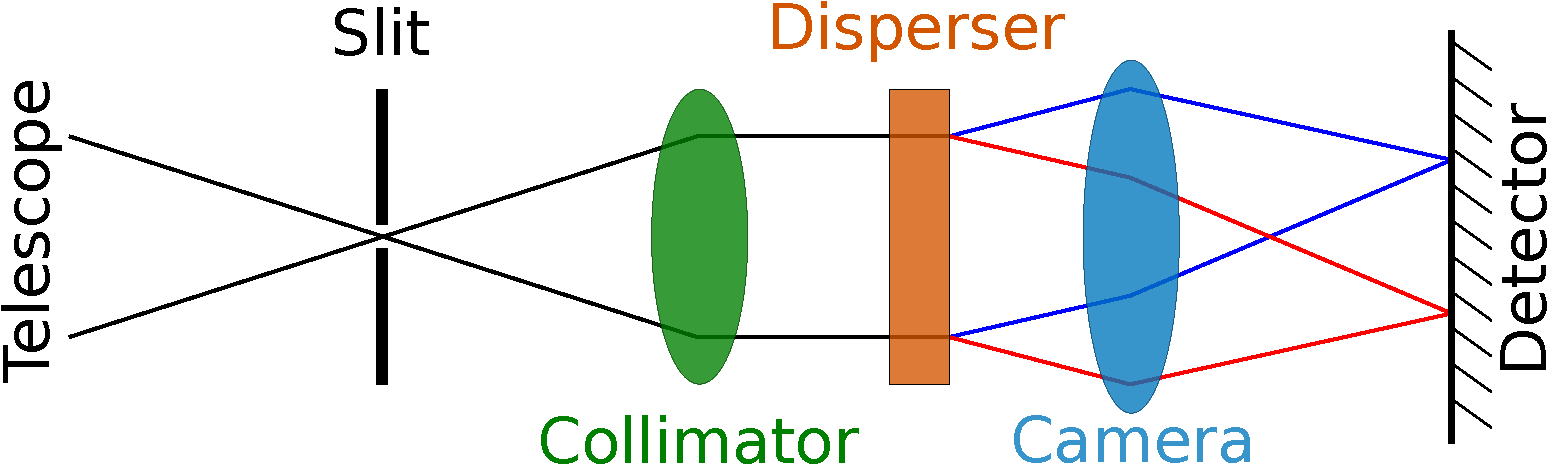
\includegraphics[width=0.7\linewidth]{figures/spectroscopy/spectrograph_elements}
    \caption{Diagram of the basic components of a spectrograph.}
    \label{fig:spectrographelements}
\end{figure}
A spectrograph is a instrument of measuring the electromagnetic flux as a function of wavelength.
All spectrographs have a few basic components common to all.
A simple diagram with the basic components is shown in \cref{fig:spectrographelements}.
The first is the telescope which is used to collect light and focus the image of the sky onto its focal plane.
A slit (or an optical fibre\footnote{Fibres allow for the spectrograph to be situated far from the telescope.}) is placed on the telescopes' focal plane to block all but the light from desired target.
The light passing through the slit is diverging so a collimator is used turn the diverging light into a parallel beam.
The dispersing element is next and is responsible for dispersing the light into its separate components.
This can be either a prism, grating (or even both).
Following the dispersive elements are the optics for the camera, used to focus the dispersed (but still fairly collimated) light onto the detector, commonly a two-dimensional array of light sensitive pixels situated at the focal plane.
Usually several optical elements, both lenses and mirrors, are used in combination to meet the constraints of the design specifications.

Figure \cref{fig:dispersion_elements} shows the schematic for 3 different dispersions mechanisms, the refraction of light due to a change (Snells law) a transmission grating and a reflection grating.
\begin{figure}
    \centering
    \begin{tabular}{ccc}
   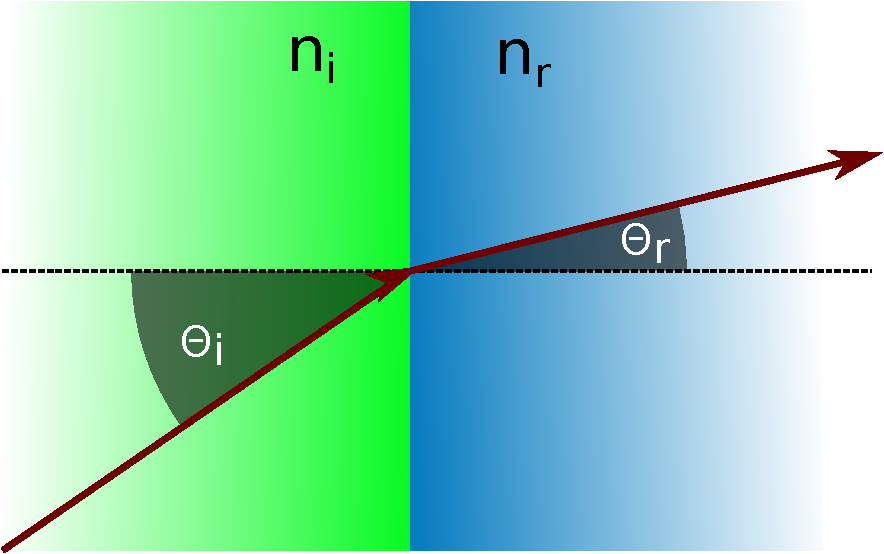
\includegraphics[width=0.3\linewidth]{figures/spectroscopy/snells_law} & 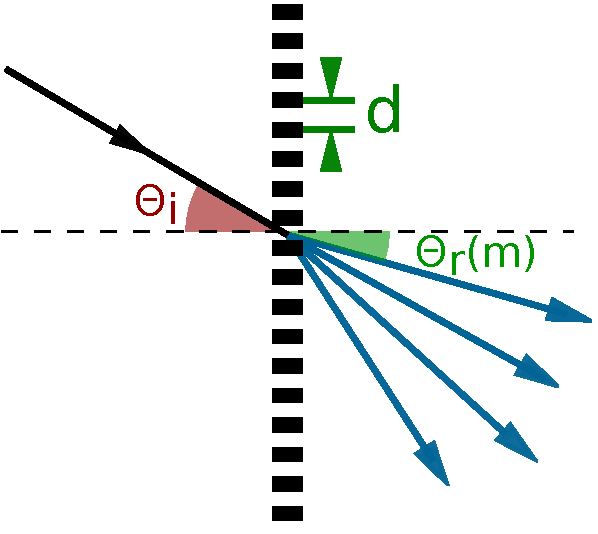
\includegraphics[width=0.2\linewidth]{figures/spectroscopy/dispersion_grism-transmission} & 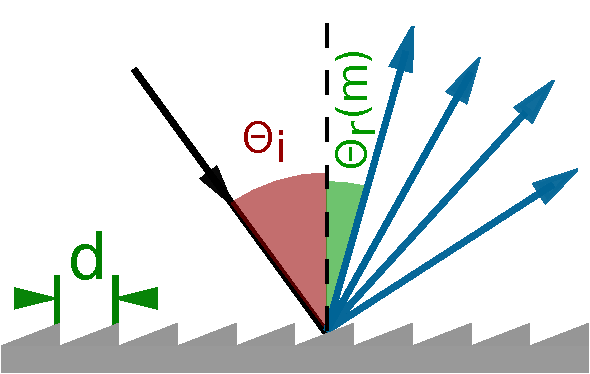
\includegraphics[width=0.3\linewidth]{figures/spectroscopy/dispersion_grism-reflection} \\
\end{tabular}
    \caption{Left: Dispersion at an optical boundary due to Snell's law.
        Middle: Dispersion from a transmission grating.
        Right: Dispersion from reflection grating.}
    \label{fig:dispersion_elements}
\end{figure}
The left hand picture depicts in which refraction of light occurs when passing between two materials of different refraction index, $n_{i}$, and $n_{r}$.
The angle of incidence $theta_{i}$ and angle of refraction $\theta_{r}$ relative to the normal (perpendicular) of the surface are related through Snell's law:
\[n_{i} \sin(\theta_{i}) = n_{r} \sin(\theta_{r}).\]
The index of refraction of a material is wavelength dependant the angle of refraction will be different for each wavelength, causing dispersion, like a prism.

The two dispersion gratings in \cref{fig:dispersion_elements} are comprised of parallel narrow slits (transmission) or grooves (reflection), very close together.
Diffraction from these slits/groves constructively and destructively interfere to create spectral orders that obey the grating equation:
\begin{equation}
m \lambda = d [\sin(\theta_{i}) \pm \sin(\theta_{r})].
\end{equation}
Here $m$ is the order number, $\lambda$ the wavelength, d the spacing between the slits/grooves, and again $\theta_{i}$ and $\theta_{r}$ the incident and reflection angles respectively, relative to the normal.

This equation has degeneracy as different combinations of $m \lambda$ will be dispersed at the same angles.
For instance the value $m \lambda$ for order $m$=54 at $\lambda$=2100\nm{} is that same as to order $m$=55 at $\lambda$=2061.8\nm{}.
This degeneracy can be overcome in two ways, either apply a wavelength filter to specifically select only one order or by adding a cross-disperser.
A \emph{cross-disperser} is a second dispersive element oriented to disperse the orders perpendicular to the grating.
This allows for multiple orders to recorded simultaneously on a two-dimensional detector, dramatically increasing the wavelength coverage.
Echelle spectrographs are a special type of spectrograph, with a groove shape and orientation specifically for high reflection angles, and to observe at a high spectral order (high $m$) to achieve a high dispersion and high resolution.

Some important concepts for discussing spectrographs are the spectral resolution, resolving power, spectral coverage and spectral sampling.
The spectral resolution, \(\delta \lambda\), is smallest difference in wavelength able to be identified.
It is related to resolving power which is defined as \(R=\frac{\lambda}{\delta\lambda}\).
The resolving power, R is colloquially also referred to as the resolution\footnote{This document is no different.} The higher the resolution (resolving power), R, the smaller the \(\delta\lambda\) that can be measured, leading to a high sampled spectral lines and more precise measurement.
To be considered high-resolution, spectrographs typically have \(R>20\,000\), but the definition of ``high'' can differ between sub-fields of astronomy.
The spectral coverage is the range of wavelengths able to be covered by the spectrograph, while the spectral sampling is the number of pixels required to sample the {FWHM} of the spectral lines.
This value should be higher than 2 pixels per resolution element to satisfy Nyquist sampling.

\section{The detectors}
\label{subsec:nir_detectors}
The basic principles of spectroscopy are the same for optical and infrared are the same one difference is the design of the detector.
Nowadays the most common type of detector are focal plane arrays, a two-dimensional of pixels located at the focal plane of the spectrographs camera.
The purpose of the detector is to count the number of photons hitting each pixel in the array.
This is achieved via the photoelectric effect on a crystalline structure, in which incident photons are transformed into electrons which can be recorded electronically.
The energy necessary to excite an electron from the \emph{valence band} to the \emph{conduction band}, the characteristic band gap, is different for every material.
Silicon is the best material for the detection of optical light (0.3--1.1\um), while in the near-infrared (1--5\um) two materials are used: {Mercury-Cadmium-Telluride} (\si{HgCdTe}) and {Indium Antimonide} (\si{InSb}).
In the mid-infrared (5--20\um) arsenic doped Silicon is used (\si{Si}:\si{As}).

Since photon energy is inversely proportional to wavelength\footnote{\(E_{photon} = \frac{h c}{\lambda}\), where $c$ is the speed of light, $h$ is Plank's constant and $\lambda$ wavelength.}, longer wavelength must have smaller band gaps.
However, smaller band gaps are also more susceptible to electrons excited by thermal energy, known as the dark current.
The dark current is dependant on detector temperature, the pixel size, quality of material and the materials cut-off wavelength $\lambda_c$.
A summary of values for different material properties is given in \cref{tab:semiconductor_properties}.

\begin{table}
    \centering
    \caption{Properties of popular optical/{IR} detector materials.
        \(\epsilon_{g}\) is the material band gap, the minimum excitation energy.
        $\lambda_c$ is the cut-off wavelength corresponding to the maximum wavelength for each material.
        Common values for the detector operating temperature for the materials is given as $T_{op}$.}
    \begin{tabular}{lcccc}
        \toprule
        Material & Symbol & $\epsilon_{g}$[eV] & $\lambda_c$[\um] & $T_{op}$[\K]\\
        \midrule
        Silicon & \si{Si} & 1.12 & 1.1 & 163-300 \\
        Mer-Cad-Tel & \si{HgCdTe} & 0.09-1.00 & 1.24-14& 20-80\\
        Indium Antimonide & \si{InSb} & 0.23 & 5.5 & 30 \\
        Arsenic doped Silicon & \si{Si}:\si{As} & 0.05 & 25 & 4 \\
        \bottomrule
    \end{tabular}\label{tab:semiconductor_properties}
\end{table}

\begin{figure}
    \centering
    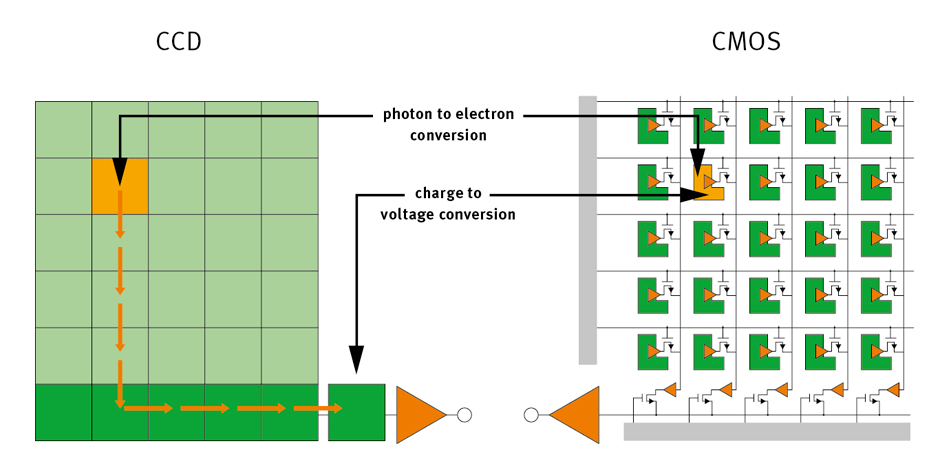
\includegraphics[width=0.8\linewidth]{figures/spectroscopy/CMOS-vs-CCD-schema}
    \caption{Schema differentiating {CCD} and {CMOS} detectors.
In {CCDs} the charge is transferred to a specific pixel for measurement while in {CMOS} the charge is measured at the location of each pixel by individual amplifiers and {ADCs}.
Credit \href{https://automatie-pma.com/pma/innovatie-en-technologie-pma/cmos-vervangt-steeds-meer-hoogwaardige-ccd-toepassingen/}{https://automatie-pma.com}.}
    \label{fig:cmos-vs-ccd-schema}
\end{figure}

The technologies for optical and {IR} detectors are very different.
\Cref{fig:cmos-vs-ccd-schema} shows the main architectural difference between {CCD} and {CMOS} is given, with a very brief comparison between them below.
Charge-Coupled Devices ({CCDs}) are used in the visible.
Their use of silicon allows for the photo-induced electrons to methodically transfer the charge be from pixel to pixel along to one end.
The electrons from each pixel pass to into amplifier to increase the signal, and then measured as a voltage difference with an analogue-to-digital converter (ADC).
As the charge is shifted between pixels {CCDs} require high charge transfer efficiency (CTE) to not leave charge behind, which would be assigned to the incorrect pixels.
{CCDs} have an almost 100\% filling of photosensitive material.
However the $\lambda_c$ cut-off of silicon makes them unsuitable for the {IR}.
More information on {CCDs} can be found in~\citep{howell_handbook_2000}.

For {IR} the technology of choice is {CMOS} (Complementary Metal Oxide Semiconductor).
Unlike {CCDs}, each individual pixel contains the circuity to read and amplify measure the charge in itself.
Since the charge is read and amplified at each pixel there is no charge transfer between pixels and the readout is non-destructive.
As a consequence, the same pixel can be read several times, averaging and thus reducing the effective readout noise of each pixel.
In theory, if one average $N$ measurements before an observation (of a freshly reset detector), and $N$ measurements of the observed charge after integration, the readout noise can be reduced by a factor of $\sqrt{(N)}$, referred to as \emph{Fowler Sampling}~\citep{fowler_demonstration_1990}.
Reading a {CMOS} detector is very versatile as it can be read in multiple ways, with the ability to randomly read any pixel at any time.
The filling area of the photosensitive material is reduced in {CMOS} due to the presence of support architecture that is required for the circulation the top surface, partially blocking some of the incident light, reducing their efficiency.

As it is impossible to have every individual amplifier perfectly identical amplifier, there is a small sensitivity and gain difference between {CMOS} pixels, which are exposed by calibrating with a uniform light source.
This contrasts with the one or few amplifiers used in CCDs, which lead to extremely homogenous amplification (as all pixels are amplified by the same amplifier).
The {CMOS} circuitry is also intrinsically non-linear due to the changing capacitance as charge is collected.
Irrespective if the charge is photo-induced or dark current, the circuitry measurement changes with the pixel charge level.
This requires careful characterization of the non-linearities in the detector by calibrating its response to a uniform light source for a large range of integration times.
For CRIRES there are a set of non-linearity coefficients that are applied while performing the flat-field corrections (see \cref{subsubsec:flat-field}).

Other benefits of {CMOS} detectors are that they use lower power, and do not need a mechanical shutter (they can be reset electronically).
While {CCDs} have been manufactured almost the same way for the last 40 years, {CMOS} technology is still advancing, partially driven by the consumer electronics market.
Nowadays, most cellphone and laptop cameras use {CMOS} chips, helping to push investment in this technology.
After the charge has been digitized into a number, the processes once again similar for both technologies.

\subsection{Spectrograph cooling}
\label{subsec:cold_spectrogrpah}
Spectrographs must be cooled down for their detectors operate effectively as seen in \cref{tab:band_ranges}.
This is achieved by placing spectrographs and their supporting components inside a vacuum chamber, away from all warm (radiating) component and precisely cooled\footnote{Temperature stability in the milli-\K range.} to low temperature.
These are often referred to as cryostat's.
Modern instruments use closed-cycle refrigerators, with for example, helium as the working fluid to achieve very stable low temperatures inside the cyrostat.
Providing a isolated, and stable environment for the spectrograph allows spectra science to be performed with the high precision possible, essential for detecting and charactering exoplanets.

Cooling plays two important roles for {IR} astronomy.
Firstly, the thermal infrared emission from the components of the spectrograph surrounding the detector is reduced, diminishing the local background.
Secondly, the detectors own thermally-generated background (dark current) is greatly reduced at low temperatures, leading to a gain in sensitivity.

Examples of two cryostat housings surrounding the spectrograph (but shown open) can be seen below in \cref{fig:nirps-vs-spirou}.


\section{CRIRES}
\label{sec:CRIRES}
CRIRES (Cryogenic InfraRed Echelle Spectrograph) is an ESO {IR} spectrograph that was mounted on the Unit Telescope (UT1, Autu) of the European Southern Observatory's Very Large Telescope (VLT)~\citep{kaeufl_crires_2004} and available from April 2007 through July 2014\footnote{Note this PhD research began in October 2014.}.
The main optical elements consist of a prism pre-disperser and a 31.6\,lines/mm echelle grating.
The instrument provides resolutions up to 100\,000 when used with a 0.2$\matharcsec$ slit\footnote{The rule of thumb for the resolution of CRIRES is \(R=100\,000 \times \frac{\textrm{slit width}}{0.2\matharcsec}\), with the slit width in arcseconds.}.
The wavelength range is 960--5200\nm{} with an instantaneous wavelength coverage of \(\sim \lambda/50\).
The spectra are imaged on a detector mosaic, consisting of four Aladdin III detectors (\(4096 \times 512\) pixel) in a row, with a gap of \(\sim 250\) pixels between each chip.
Adaptive optics (MACAO - Multi-Applications Curvature Adaptive optics) can be used to optimize the signal-to-noise ratio and the spatial resolution.
\Cref{fig:criresschematic} displays the schematic representation of the CRIRES optical layout.

CRIRES lead the way for high-resolution spectrograph in the {IR} with a resolution higher than any of its predecessors, and unique capabilities, like adaptive optics.
As with any new instrument there were several problems that affected CRIRES during its science operations.
For instance there were several mechanical issues with the slit; the slit edges were not parallel and there were issues with precise and reproducible positioning.
Other issues that require post observation correction such as detector glow, the odd even effect, and the wavelength calibration are detailed in \cref{subsubsec:darkcurrent,subsubsec:flat-field,subsec:wavecalib}.

\begin{figure}
    \centering
    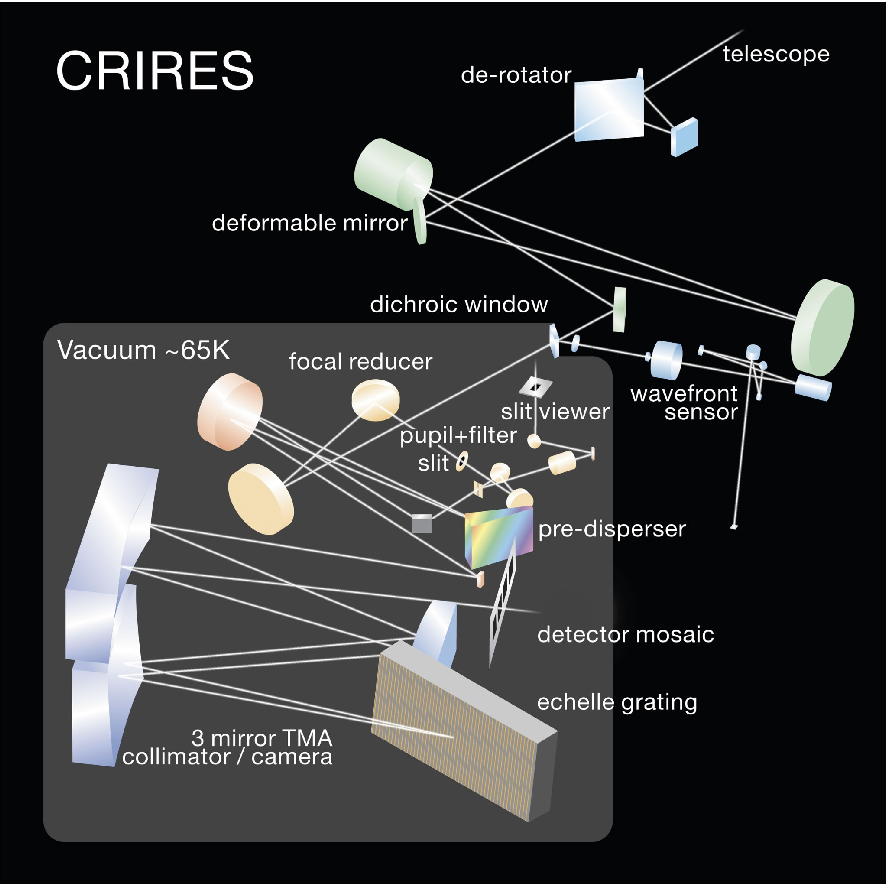
\includegraphics[width=0.7\linewidth]{figures/spectroscopy/CRIRES_schematic.pdf}
    \caption{CRIRES layout schematic, taken from the CRIRES manual v93.}
    \label{fig:criresschematic}
\end{figure}


\section{The new generation}
\label{subsec:new_generation}
Building off the success of CRIRES several other \nir{} spectrograph have and being developed for different telescopes.

Their science goals for these instruments involve some or all of the following:

\begin{itemize}
\item Detecting low-mass planets in the habitable zone around late-type stars (M-dwarfs).
\item Detecting and characterising the atmospheres of exoplanets.
\item Observe and monitor clouds on brown dwarfs.
\item Analysing the spectra and atmospheres of cool stars.
\item The origin and evolution of stellar magnetic fields (through spectropolarimetry).
\end{itemize}

A few points about some of the \nir{} instruments used in this work are detailed below with a summary also provided in \cref{tab:insturment_summary}.

\begin{table}
    \caption{A comparison between some high-resolution \nir{} spectrographs.}
    \begin{tabular} {lcccc}
        \toprule
        & {CRIRES+} & {CARMENS} (red) & {NIRPS} & {SPIRou}\\
        \midrule
        \multirow{2}*{Location} & Paranal, & Calar Alto, & La Silla, & Mauna Kea,\\
              &  Chile & Spain & Chile & Hawaii \\
        Latitude & \(24^\circ 40^\prime\) S & \(37^\circ 13^\prime\) N & \(29^\circ 15^\prime\) S & \(19^\circ 49^\prime\) N \\
        Available (* expected) & 2019* & 2016 & 2019* & 2019* \\
        Telescope diameter (\si{\metre}) & 8.2 & 3.5 & 3.6 & 3.6 \\
        Wavelength Range (\nm) & 920--5200 & 960--1710 & 970--1810 & 980--2350 \\
        Resolution & 50\,000/100\,000 & 80\,400 & 75\,000/100\,000 & 70\,000\\
        % Mean sampling (pixels) & & 2.8 & 3 & \textbf{1.8}??? \todo{Pedro do you have this number? from a velocity size of 2.28 km/s I think I calculate a sampling of 1.8}\\
        RV precision (\mps) & 2--3 & $\sim$1 & 1 & 1\\
        Operating Temperature (\K)& 70 & 140 & 80 & 77 \\
        %Website &\href{http://www.eso.org/sci/facilities/develop/instruments/crires_up.html}{http://www.eso.org/sci/facilities/develop/instruments/crires\_up.html} & \href{carmenes.caha.es}{carmenes.caha.es} & \href{http://www.astro.umontreal.ca/nirps/}{http://www.astro.umontreal.ca/nirps/} & \href{}{}\\
        \bottomrule
    \end{tabular}\label{tab:insturment_summary}
\end{table}

\todo{Is there other properties I should add to \cref{tab:insturment_summary}}

\subsection{CRIRES+}
\label{subsec:criresplus}
CRIRES was removed from operation in 2014 to undergo significant upgrades~\citep{dorn_crires_2014}.
These include adding a cross-disperser to increase the simultaneous wavelength coverage by up to a factor of 10, improving the wavelength calibration by replacing the \thar{} calibration lamp with a \une{} lamp which has a richer set lines in the IR, and developing new multi-species gas absorption cells for the {IR}.
The new upgrade adds the capability for spectropolarimetry using a polarization selective beam-splitter, in which the polarization of light in the spectrum can be analysed.
The current detector mosaic will be replaced by 3 Hawaii 2RG detectors (\(6144\times 2048\) pixels) at a pixel size of 18\um{}.
A comparison between the new and old detector size is shown in \cref{fig:criresplus_detecotrs}.
The new detector mosaic will not only provide a larger area but also lower noise, higher quantum efficiency, better cosmetic quality and much lower dark current
\footnote{\href{https://www.eso.org/sci/facilities/develop/instruments/crires_up.html}{https://www.eso.org/sci/facilities/develop/instruments/crires\_up.html}}.
The current estimate for the first light of CRIRES+ is first quarter of 2019.

\begin{figure}
    \centering
    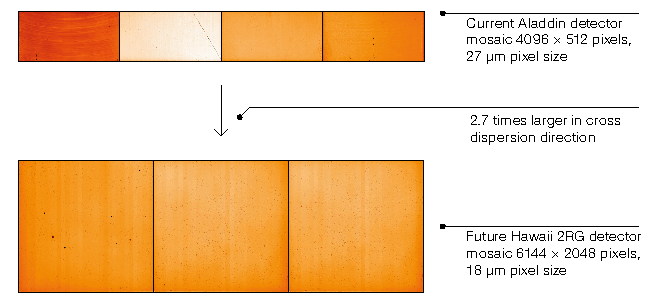
\includegraphics[width=0.5\linewidth]{figures/spectroscopy/criresplus_detectors.pdf}
    \caption{CRIRES detector focal plane array comparison with the new detectors.
    Credit~\citet{dorn_crires_2014}.}
    \label{fig:criresplus_detecotrs}
\end{figure}

\subsection{CARMENES}
\label{subsec:carmenes}
{CARMENES} (Calar Alto high-Resolution search for M dwarfs with Exoearths with Near-infrared an optical \'Echelle Spectrographs) has been operating since 2016, performing an dedicated RV survey of \(\sim300\) late-type main-sequence stars with the goal of detecting low-mass planets in the habitable zone.
It is mounted on the 3.5\m{} telescope at the Calar Alto Observatory in Spain, the light from the telescope is passes through a beam splitter and enters into two separate spectrographs, one in the optical (520--960\nm{}) and the other in the infrared (960--1710\nm{}).
A library of single spectra of the {M-dwarf} targets CARMENES is monitoring was recently released in~\citep{reiners_carmenes_2018}.

\subsection{NIRPS}
\label{subsec:nirps}
{NIRPS} (Near-InfraRed Planet Searcher) is a \nir{} extension to the {HARPS} spectrograph on the 3.6\m{} telescope at La Silia, Chile.
One of the most prominent spectrographs detecting exoplanets via a RV method.
A replacement for the {HARPS} telescope adapter will be used to split the light and send the optical wavelengths to {HARPS} and {IR} to {NIRPS} via fibres.
The adaptor also includes adaptive optics and a new calibration unit.

This will allow for the RV monitoring of cooler stars which, emit more of their photons in the infrared but also have less stable optical spectra due to convection; infrared spectra are less affected by the stellar activity.

\subsection{SPIRou}
\label{subsec:spirou}
{SPIRou} (SPectroplorim\`etre InfraROUge) is another high-resolution \nir{} spectrograph that will be installed at the {CFHT} (Canada-France-Hawaii Telescope) in Hawaii.
It will provide a spectrum covering from 950--2340\nm{} in a single exposure at a resolution of around \(\sim75\,000\).
Like the other spectrographs detailed here it is built to obtain very high radial velocity accuracy, of the order meters/second over several year.
It also includes spectropolarimetry, being able to derive the linear and circularly polarized state of the observed target.

A physical side-by-side comparison of the {NIRPS} and {SPRIou} spectrographs is shown in \cref{fig:nirps-vs-spirou}, with {NIRPS} towards the front left.
\begin{figure}
    \centering
    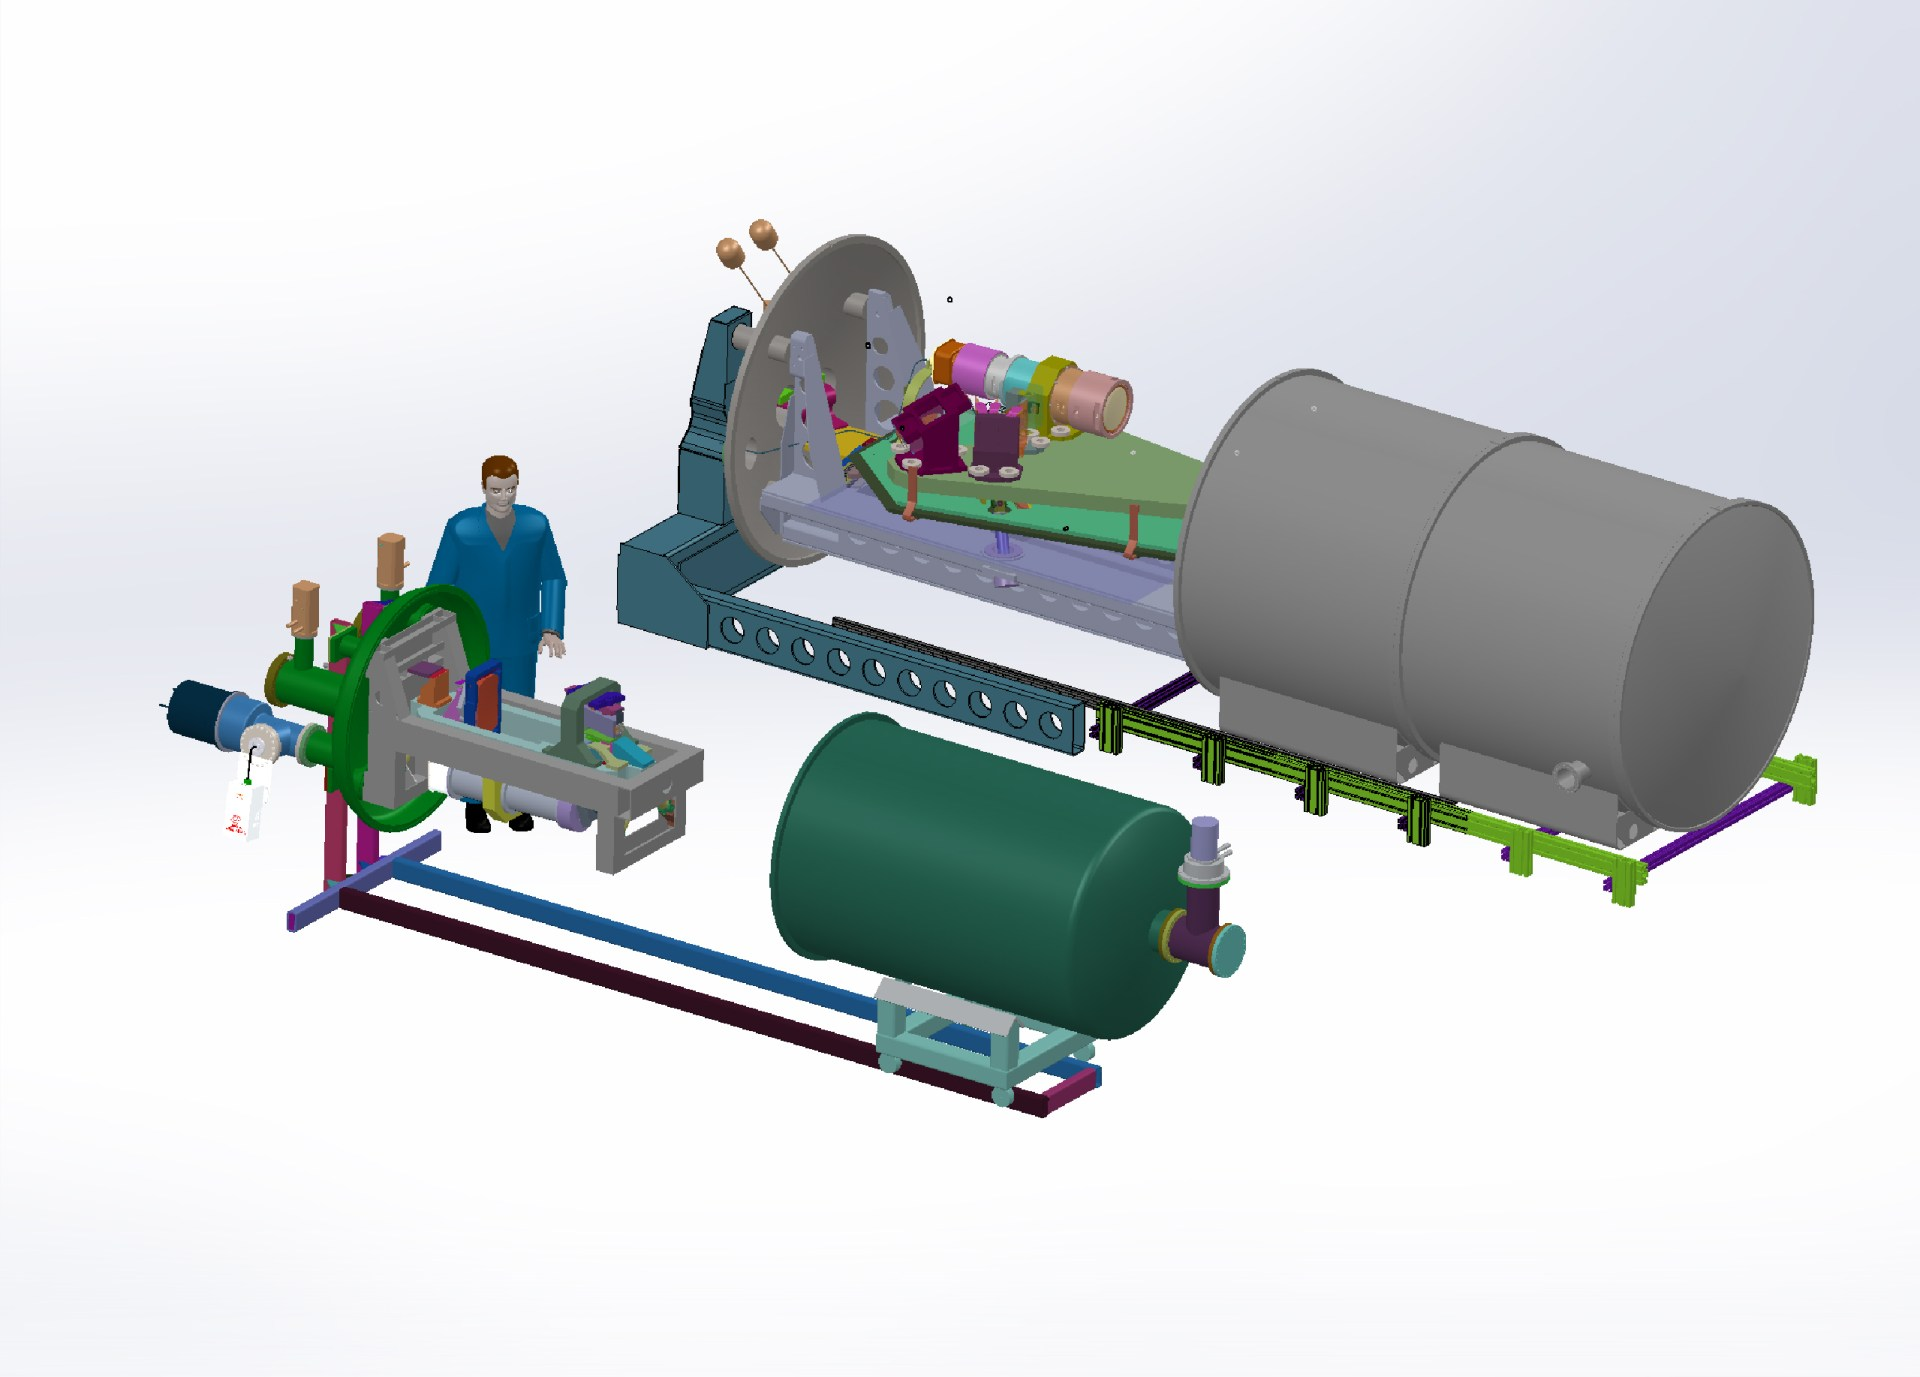
\includegraphics[width=0.7\linewidth]{figures/spectroscopy/NIRPS-vs-SPIROU}
    \caption{Side by side comparison of the {NIRPS} and {SPIRou} spectrographs.
        {NIRPS} is the one in front on the left.
        Credit \href{http://www.astro.umontreal.ca/nirps/}{http://www.astro.umontreal.ca/nirps/}.}
    \label{fig:nirps-vs-spirou}
\end{figure}


\todo{the Atmopshere in the nir}
